\documentclass[11pt,a4paper]{article}
 
\usepackage[T1]{fontenc}
\usepackage[portuguese]{babel}
\usepackage{authblk}
\usepackage{enumitem}
\usepackage{graphicx}



\pagenumbering{arabic}

\setlist[description]{labelindent=1cm}

\title{\textbf{Projecto de Base de Dados}}
 
\author{Bruno Cardoso e Lidia Freitas e Rodrigo Bernardo} 

\affil{Instituto Superior T\'{e}cnico}
 
\date{Parte 1}
 
\begin{document}
\setlength{\pdfpxdimen}{1in/250}
\maketitle

\newpage
\setcounter{page}{1}

\tableofcontents %Índice de conteúdos
\newpage
\section{O Modelo}
\subsection{Modelo Entidade-Associa\c{c}\~ao}



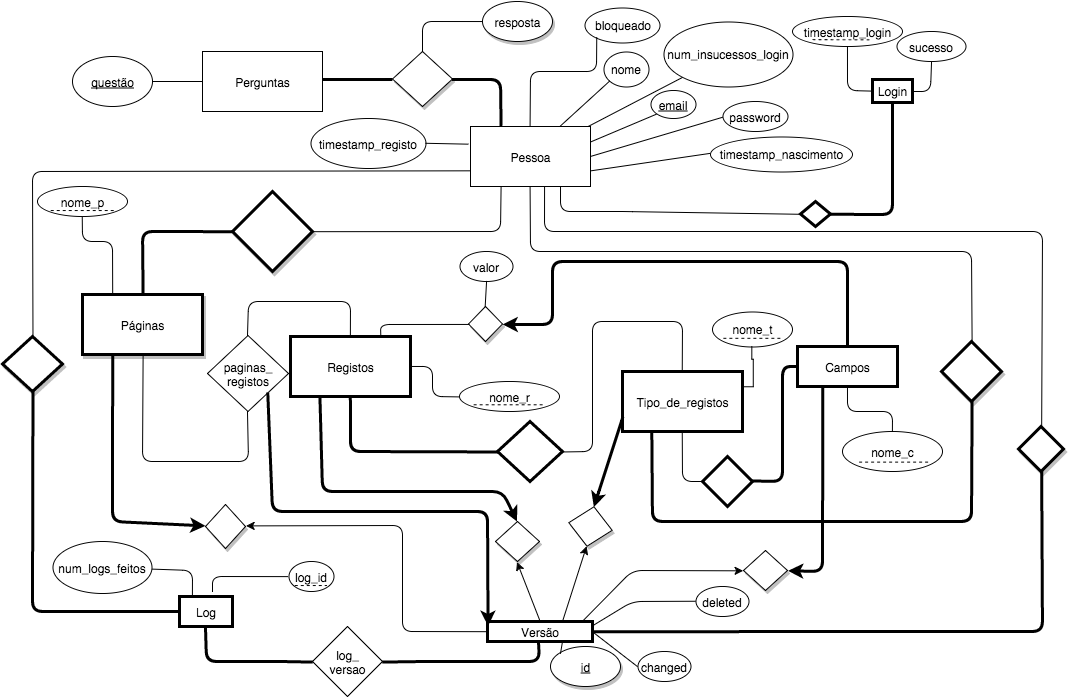
\includegraphics[scale=0.48]{modelo-ea.png}


ADICIONAR CHAVE CANDIDATA A PESSOA.(Alternativa de entrar na conta)
\newpage
\subsection{Restri\c{c}\~oes de Integridade do Modelo Entidade-Associa\c{c}\~ao}

\paragraph{}

O Modelo Entidade-Associa\c{c}\~{a}o, apenas com o diagrama, n\~{a}o exige que n\~{a}o ocorram situa\c{c}\~{o}es fora do dom\'{\i}nio do problema.




\section{Modelo Relacional}
\subsection{O Modelo}

\begin{description}[noitemsep]
	\item Pergunta(\underline{quest\~ao, email}, resposta)
	\item email: FK(Pessoa)
	\item notnull(resposta)
\end{description}

\begin{description}[noitemsep]
	\item Pessoa(\underline{email}, bloqueado, nome, insucesso, password, timestamp\_nascimento, timestamp\_registo)
	\item nutnull(email,bloqueado, nome, insucesso, password, timestamp\_nascimento, timestamp\_registo)
\end{description}

\begin{description}[noitemsep]
	\item Login(\underline{timestamp\_login, email}, sucesso)
	\item email: FK(Pessoa)
	\item notnull(sucesso)
\end{description}

\begin{description}[noitemsep]
	\item P\'{a}ginas(\underline{email, nome\_p}, id)
	\item email: FK(Pessoa)
	\item id: FK(Pessoa)
	\item notnull(id)
	\item unique(id)
\end{description}

\begin{description}[noitemsep]
	\item P\'{a}ginas\_registos(\underline{nome\_p, email, nome\_r})
	\item email: FK(Pessoa)
	\item nome\_p: FK(P\'{a}ginas)
	\item nome\_r: FK(Registos)
\end{description}

\begin{description}[noitemsep]
	\item Registos(\underline{nome\_r, nome\_t}, id)
	\item nome\_t: FK(Tipo\_de\_registos)
	\item unique(id)
	\item notnull(id)
	\item id: FK(Vers\~{a}o)
\end{description}

\begin{description}[noitemsep]
	\item Tipos\_de\_registos(\underline{nome\_t, email}, id)
	\item email: FK(Pessoa)
	\item notnull(id)
	\item unique(id)
	\item id: FK(Vers\~{a}o)
\end{description}

\begin{description}[noitemsep]
	\item Campos(\underline{nome\_c, nome\_t, nome\_r}, valor, id)
	\item nome\_t: FK(Tipo\_de\_registos)
	\item nome\_r: FK(Registos)
	\item notnull(id)
	\item unique(id)
\end{description}

\begin{description}[noitemsep]
	\item Vers\~{a}o(\underline{id}, changed, deleted)
	\item notnull(changed)
	\item notnull(deleted)
\end{description}

\begin{description}[noitemsep]
	\item Log(\underline{log\_id, email})
	\item email: FK(Pessoa)
\end{description}

\begin{description}[noitemsep]
	\item Log\_vers\~{a}o(\underline{log\_id, id})
	\item log\_id: FK(log)
	\item id: FK(Vers\~{a}o)
\end{description}








\subsection{Restri\c{c}\~oes de Integridade do Modelo Relacional}
\section{\'{A}lgebra Relacional}
\subsection{Pergunta 1}
\subsection{Pergunta 2}
\subsection{Pergunta 3}
\subsection{Pergunta 4}

\section{Linguagem SQL}
\subsection{Pergunta 1}
\subsection{Pergunta 2}
\subsection{Pergunta 3}
\subsection{Pergunta 4}

\end{document}